\documentclass[10pt]{article} % For LaTeX2e
\usepackage{tmlr} % anonymous submission mode (authors auto-hidden)
\usepackage{hyperref}
\usepackage{url}

\usepackage{amsmath,amssymb,amsthm}
\usepackage{booktabs}
\usepackage{microtype}
\usepackage{graphicx}
\usepackage{titlesec}
% run-in paragraph headers in italic, not bold
\titleformat{\paragraph}[runin]{\normalfont\itshape}{}{0pt}{}
\titlespacing*{\paragraph}{0pt}{0.6\baselineskip}{0.6em}

\newtheorem{proposition}{Proposition}
\newtheorem{corollary}{Corollary}
\newtheorem{lemma}{Lemma}
\theoremstyle{definition}
\newtheorem{definition}{Definition}
\newtheorem{remark}{Remark}

\newcommand{\R}{\mathbb{R}}
\newcommand{\E}{\mathbb{E}}
\renewcommand{\Pr}{\mathbb{P}}
\newcommand{\KL}{\mathrm{KL}}
\newcommand{\given}{\,\vert\,}
\DeclareMathOperator*{\argmax}{arg\,max}

\title{Marginally Useful:\\ Formalizing the Information Gap in Conformal Prediction}

% Authors are hidden automatically in submission mode (no [accepted]/[preprint] option).
\author{\name Anonymous \email anonymous@example.com \\
        \addr Anonymous Institution}

\begin{document}
\maketitle

\begin{abstract}
Conformal prediction gives finite-sample, distribution-free \emph{marginal} coverage for a
set. The guarantee is real, and it is often misread as evidence of forecast quality. We
separate the two with one decomposition, the residual-information gap: for a fixed location
predictor and a single-shape residual predictive system, the log-score regret relative to the
oracle is exactly the mutual information $I(R;X)$ between the residual and the input.
Conformalization re-levels coverage but cannot touch this quantity, because it is a property
of the predictor's shape class and not of calibration; no recalibration that ignores $X$
reduces it within that class. The familiar cautions about conformal prediction follow as context: marginal coverage is
not conditional, validity is insensitive to sharpness, and the guarantee needs
exchangeability.
\end{abstract}

\section{Introduction}

A practitioner maintains a probabilistic forecaster and is told, repeatedly, that
conformal prediction is the principled, distribution-free way to ``add uncertainty.''%
\footnote{The reading is pervasive. Applied and survey writing routinely calls the
marginal-coverage guarantee ``well-calibrated'' or ``reliable'' uncertainty quantification
\citep{bellotti2025trustworthy}, and tutorials present conformal prediction as the way to
``add uncertainty'' \citep{tds_adduncertainty} or to ``predict full probability
distributions'' \citep{manokhin_fulldist}. The methodological literature is more careful,
separating \emph{validity} from \emph{efficiency}, and a critique strand makes the present
point independently \citep{pitfalls2025medical,min2026coveragelength}. Our quarrel is with
the conflation, not with conformal prediction.}
They bolt it on. The number they actually report (a proper score such as the
predictive log-likelihood) does not improve. The natural diagnosis is a tuning
failure. The real one is a \emph{category error}: conformal
prediction is a method for \emph{certifying the coverage of a set}, and it is being
asked to \emph{estimate a distribution}. These are different kinds of object, graded
by different instruments, and no amount of tuning turns one into the other. None of
this is a criticism of the method. It is a guide to where the method belongs.

The mathematics is not in question. Given exchangeable data, a fitted predictor,
and a nonconformity score, split conformal prediction returns a set $C_\alpha(x)$ with
\begin{equation}\label{eq:marginal}
  \Pr\!\big(Y_{n+1}\in C_\alpha(X_{n+1})\big)\;\ge\;1-\alpha,
\end{equation}
finite-sample and with no assumption on the data distribution
\citep{vovk2005algorithmic,lei2018distribution,angelopoulos2023gentle}. The trouble
is entirely in the reading of \eqref{eq:marginal}. The probability averages over
$X_{n+1}$ as well as $Y_{n+1}$: it is a statement about the \emph{average} future
input, not about the one in front of you. It is \emph{marginal} coverage, and as the
foundational analyses warned from the start, ``a good estimator must satisfy something
more than marginal coverage'' \citep{lei2014distribution}.

\paragraph{Contributions and structure.}
The one new result is in Section~\ref{sec:gap}: for a single-shape residual predictive
system, the log-score regret to the oracle equals the mutual information $I(R;X)$ between
the residual and the input, and no recalibration that ignores $X$ can reduce it
(Proposition~\ref{prop:gap}). We call this the residual-information gap.

The other sections are background and consequences. The impossibility of distribution-free
conditional coverage (Section~\ref{sec:marginal}) is due to \citet{lei2014distribution} and
\citet{barber2021limits}. The orthogonality of coverage and log-score
(Section~\ref{sec:orthogonality}) is folklore. The coverage--score plane
(Section~\ref{sec:plane}) is a way of presenting the result. Section~\ref{sec:exch} covers
exchangeability and time series, Section~\ref{sec:steel} the case where coverage is the
objective, and Section~\ref{sec:scope} the relation to the modern conformal literature.

\section{Setup: split conformal and the marginal guarantee}\label{sec:setup}

Let $(X_i,Y_i)_{i=1}^{n+1}$ be exchangeable. Fix a point predictor $\hat\mu$ trained on
a disjoint set, and a \emph{nonconformity score} $s(x,y)$; the canonical choice in
regression is the absolute residual $s(x,y)=|y-\hat\mu(x)|$. Compute calibration
scores $s_i=s(X_i,Y_i)$ for $i=1,\dots,n$ and let
\begin{equation}\label{eq:q}
  \hat q \;=\; s_{(k)}, \qquad k=\big\lceil (n+1)(1-\alpha)\big\rceil,
\end{equation}
the $k$-th order statistic (with $\hat q=+\infty$ when $k>n$). The split-conformal set is
\begin{equation}\label{eq:set}
  C_\alpha(x)=\{y:\ s(x,y)\le \hat q\}
  \;=\;[\hat\mu(x)-\hat q,\ \hat\mu(x)+\hat q]
\end{equation}
for the absolute-residual score. Exchangeability of the augmented scores makes the rank
of $s_{n+1}$ uniform, which yields \eqref{eq:marginal}
\citep{vovk2005algorithmic,lei2018distribution}. The construction is simple and the
guarantee is real, and one readily verifies that empirical coverage tracks $1-\alpha$ as
the sample size, noise level, and $\alpha$ are varied. None of this is in dispute. The
question is what it is taken to mean.

\section{Three known limits of the marginal guarantee}\label{sec:marginal}

None of the three facts below is new. We restate them, with attribution, to fix notation
and to mark where the contribution of Section~\ref{sec:gap} departs from what is already
established.

\paragraph{(i) Marginal is not conditional, and conditional is impossible for free.}
One would prefer \emph{conditional} coverage,
$\Pr\big(Y\in C(x)\given X=x\big)\ge 1-\alpha$ for (almost) every $x$. Distribution-free,
this cannot be bought. \citet{lei2014distribution} show (their Lemma~1) that any band
with non-trivial finite-sample conditional validity has \emph{infinite} expected length
at almost every point of a continuous distribution.
\citet{barber2021limits} restate and sharpen this: a conditionally valid $C_n$ has
$\E\,\mathrm{leb}(C_n(x))=\infty$ at almost all non-atomic $x$ (their Prop.~2.2), and
even the relaxed demand of coverage on every subgroup of probability $\ge\delta$ ``is
impossible to attain beyond the trivial solution'' of inflating the marginal level to
$1-\alpha\delta$ (their Thm.~3.1). These are not loose bounds to be tightened; they are the
reason the gap cannot be closed for free, and both surface as concrete finite-sample facts.
The first is illustrated in Figure~\ref{fig:nogo}: localizing split conformal to recover
per-$x$ coverage shrinks each cell's calibration count $n_b$ until
$\lceil (n_b+1)(1-\alpha)\rceil > n_b$, at which point \eqref{eq:q} gives $\hat q=+\infty$
and the only valid cell interval is $(-\infty,\infty)$; uniform coverage is recovered only
as the fraction of infinite-length intervals grows. The second is Figure~\ref{fig:subgroup}:
the distribution-free protection of all $\delta$-subgroups is exactly the flat band at level
$1-\alpha\delta$, whose width diverges as $\delta\to 0$ while never adapting to $x$, at a
multiplicative width cost over an assumption-driven adaptive oracle.

\begin{figure}[t]
\centering
\begin{minipage}{0.49\textwidth}\centering

\includegraphics[width=\linewidth]{figures/fig_nogo.pdf}
\caption{The price of conditional coverage \citep{lei2014distribution}. As the conditioning
resolution $B$ grows, per-cell calibration sets shrink and the only valid cell interval
becomes $(-\infty,\infty)$; uniform (worst-bin) coverage is bought only as the fraction
of infinite-length intervals rises.}
\label{fig:nogo}
\end{minipage}\hfill
\begin{minipage}{0.49\textwidth}\centering
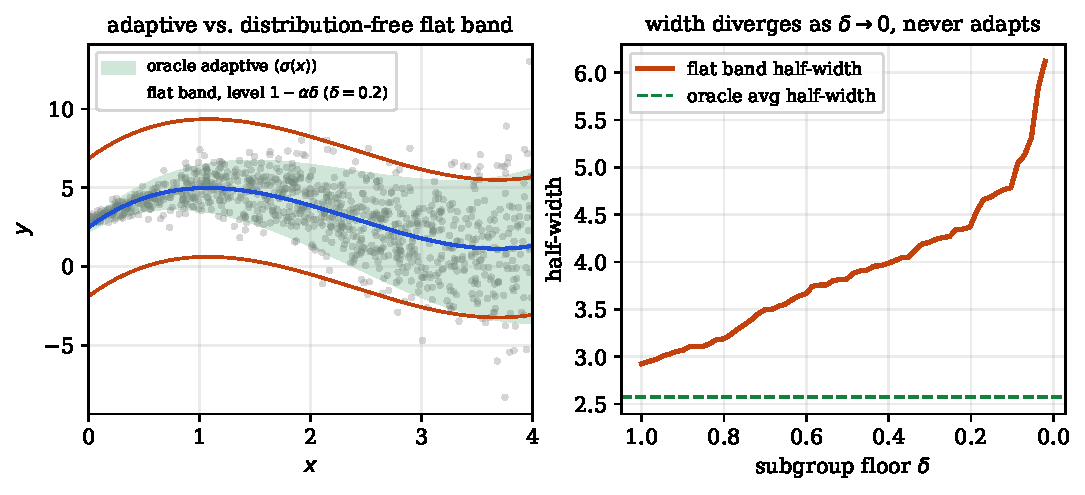
\includegraphics[width=\linewidth]{figures/fig_subgroup.pdf}
\caption{Subgroup coverage buys only a wider band \citep{barber2021limits}. The
distribution-free protection of all $\delta$-subgroups is a flat, non-adaptive band at
level $1-\alpha\delta$ whose width diverges as $\delta\to0$; the adaptive oracle that uses
$\sigma(x)$ is far tighter but requires the distributional assumption.}
\label{fig:subgroup}
\end{minipage}
\end{figure}

So the guarantee you can have distribution-free is
the marginal one, and a marginally valid band ``tends to overestimate the set when $x$
is in the high density area and to underestimate for low density $x$''
\citep{lei2014distribution}: it over-covers the easy inputs and under-covers the hard
ones, silent by construction about the cases the model was built to get right.
Figure~\ref{fig:margcond} exhibits exactly this on heteroscedastic data: $90\%$ overall,
near-$100\%$ where the noise is small, well below target where it is large.

\begin{figure}[t]
\centering

\includegraphics[width=0.92\textwidth]{figures/fig_marginal_conditional.pdf}
\caption{Marginal is not conditional. A constant-width split-conformal band (left) attains
$90\%$ \emph{marginal} coverage on heteroscedastic data, but its \emph{local} coverage
(right) runs near $100\%$ where the noise is small and well below target where it is large:
it over-covers the easy inputs and under-covers the hard ones.}
\label{fig:margcond}
\end{figure}

The conformal literature already separates \emph{validity} from \emph{efficiency}. The
point here is only that the marginal-coverage certificate does not measure distributional
quality.

\paragraph{(ii) Validity is trivially satisfiable.}
A predictor that returns the whole outcome space with probability $1-\alpha$ and the
empty set otherwise satisfies \eqref{eq:marginal} exactly and conveys nothing. More
practically, the \emph{same} coverage attaches to an excellent $\hat\mu$ and to a
deliberately terrible one; the latter merely yields a wider $\hat q$ in
\eqref{eq:q}. Marginal validity is therefore not evidence of a good method; it
certifies the fence, not the cattle. The next section makes this precise.

\paragraph{(iii) Without exchangeability, even the marginal guarantee fails.}
Equation~\eqref{eq:marginal} rests on exchangeability of the augmented sample. Under
covariate shift, label shift, or temporal dependence it does not hold, and the patches
that restore something do so by weakening what is guaranteed (Section~\ref{sec:exch}).

\section{Coverage and score are orthogonal}\label{sec:orthogonality}

We first make ``coverage is not a measure of forecast quality'' a precise, constructive
fact. Separate the two things a forecaster reports: a point predictor $\hat\mu(x)$ and a
full predictive density $f(\cdot\given x)$. The log-score grades $f$, that is, its spread
and shape, its sharpness. The canonical residual score $s(x,y)=|y-\hat\mu(x)|$ uses only
$\hat\mu$, the \emph{location} of the forecast. It never sees the spread or shape of $f$.
So the conformal set, and its coverage, are invariant to exactly the part of $f$ that the
log-score rewards. (This is specific to such scores; it does not apply to density- or
quantile-based scores, which read $f$ directly.)

\begin{proposition}[Residual-score coverage does not constrain the log-score]\label{prop:orth}
The split-conformal set \eqref{eq:set} is a measurable function of the nonconformity
scores $\{s_i\}$ and of $s(x,\cdot)$; it is not a functional of the predictive density
$f$ unless $f$ is explicitly used in the score. Consequently two forecasters with the
\emph{same} location $\hat\mu$ (hence, for the residual score, the same score function and
calibration scores) but different predictive densities $f$ have \emph{identical} conformal
sets, and identical marginal coverage at every level $\alpha$, while their expected
log-scores $\E[\log f(Y\given X)]$ may differ by an arbitrary amount.
\end{proposition}

\begin{proof}
The first claim is immediate from \eqref{eq:q}--\eqref{eq:set}: $\hat q$ is an order
statistic of $\{s_i\}$ and $C_\alpha(x)=\{y:s(x,y)\le\hat q\}$, so two forecasters
agreeing on $s$ and on $\{s_i\}$ produce the same set for every $x,\alpha$, and
\eqref{eq:marginal} concerns only that set.

For the gap, take $X$ degenerate (a point mass at an arbitrary $x_0$, i.e.\ a single
repeated input, so there is nothing to vary across) and $Y\sim N(0,1)$. Both forecasters
share the location
$\hat\mu\equiv 0$, so both use the absolute-residual score $s(x,y)=|y|$, which depends on
$\hat\mu$ but not on the spread of the predictive density. They differ only in that claimed
density, $f_\sigma=N(0,\sigma^2)$: for any $\sigma$ the scores are $|Y_i|$, independent of
$\sigma$, so the conformal set is the fixed interval $[-\hat q,\hat q]$ with $\hat q$ the
empirical $(1-\alpha)$-quantile of $|Y|$. Yet
\[
  \E[\log f_\sigma(Y)] \;=\; -\tfrac12\log(2\pi\sigma^2)-\frac{\E[Y^2]}{2\sigma^2}
  \;=\; -\tfrac12\log(2\pi\sigma^2)-\frac{1}{2\sigma^2}\;\xrightarrow[\sigma\to 0^+]{}-\infty,
\]
and likewise $\to-\infty$ as $\sigma\to\infty$. Hence for any $M>0$ there are
$\sigma_1,\sigma_2$ with identical conformal sets (identical marginal coverage at every
$\alpha$) yet log-scores differing by more than $M$.
\end{proof}

\begin{corollary}\label{cor:orth}
For a residual-score conformal predictor, marginal validity certifies an order statistic
of residual magnitudes. It does not identify, bound, or rank the scale, shape, or
sharpness of any predictive density that was not used to construct the score; in
particular, no inference about forecast quality (as graded by a strictly proper score)
can be drawn from coverage alone.
\end{corollary}

\begin{remark}[The degenerate $X$ is only for cleanliness]\label{rem:nondeg}
The point-mass $X$ in the proof makes the unbounded gap transparent, but it is not needed.
For any non-degenerate $X$, take two forecasters sharing the same location $\hat\mu$ (hence,
for the residual score, the same score function and calibration scores, so identical sets
and coverage at every $\alpha$) but predictive spreads $\sigma_1(x),\sigma_2(x)$; their
expected log-scores differ by $\E_X[\log(\sigma_2/\sigma_1)] + \tfrac12\E_X[(\sigma_2^{-2}
-\sigma_1^{-2})\,\mathrm{Var}(Y\given X)]$, which is unbounded over choices of the
$\sigma_i$. Coverage is blind to all of it.
\end{remark}

This is the formal version of a point several authors have made informally: that
conformal validity ``almost invites you to use garbage prediction functions''
\citep{recht2024cover}. Figure~\ref{fig:orth} shows it: the claimed density's spread
slides freely while the conformal interval and its $90\%$ coverage do not move, because
the spread never entered \eqref{eq:q}.

\begin{figure}[t]
\centering

\includegraphics[width=0.92\textwidth]{figures/fig_orthogonality.pdf}
\caption{Coverage does not constrain the log-score (Proposition~\ref{prop:orth}). With a
residual score the conformal set $[-q,q]$ is fixed by the outcomes alone (left), so two
predictive densities with very different log-scores share the \emph{same} set and the
same $90\%$ coverage. Sweeping the forecaster's spread $s$ (right) moves the log-score
freely while coverage stays pinned at $90\%$.}
\label{fig:orth}
\end{figure}

\section{The residual-information gap}\label{sec:gap}

Forecast quality decomposes into \emph{calibration} and
\emph{sharpness}, and the discipline's stated goal is to maximize sharpness subject to
calibration, assessed by a proper scoring rule
\citep{gneiting2007probabilistic,gneiting2007strictly}. Within the fixed-location,
single-shape residual class, signed CPS is log-score optimal; the loss is the class
restriction, not the conformal calibration step.

\paragraph{Conformal predictive systems.} A conformal predictor can be made to output a
distribution rather than a set, the \emph{conformal predictive system} (CPS) of
\citet{vovk2019nonparametric}, built from \emph{signed} residual scores. It is the mode in which conformal
prediction estimates a full distribution, so it is the form the criticism must address. We must, however, distinguish it from the more
common practice of reading the nested symmetric intervals of ordinary
\emph{absolute}-residual split conformal as if they were a distribution; the two re-level
different objects, and the distinction matters for the gap below.

\begin{proposition}[Re-leveling, two cases]\label{prop:relevel}
Fix a location predictor $\hat\mu$ with residual $R=Y-\hat\mu(X)$ of marginal density
$g$ and CDF $G$. In the large-calibration limit (under exchangeability):%
\footnote{The log-score comparison is for the limiting residual density, or equivalently a
smoothed CPS density: a finite empirical CPS is a valid predictive distribution but not
generally a Lebesgue density, so the density/log-score identity is an asymptotic (or
smoothed-density) statement. The finite-sample guarantee is coverage.}
\begin{enumerate}
\item[(A)] Signed-residual CPS. The CPS predictive distribution is
$\Pi_x(y)=G\big(y-\hat\mu(x)\big)$ (the calibration ECDF $\widehat G_n\to G$ by
Glivenko--Cantelli), with density $\pi_x(y)=g\big(y-\hat\mu(x)\big)$: the base location
forecast re-leveled by the marginal signed-residual law.
\item[(B)] Absolute-residual intervals. Ordinary split conformal at
level $\alpha$ returns the symmetric interval $\hat\mu(x)\pm \hat q_\alpha$, with
$\hat q_\alpha$ the $(1-\alpha)$-quantile of $|R|$. Read as a predictive distribution
(by sweeping $\alpha$) it is symmetric about $\hat\mu(x)$ with $|{\cdot}|$ distributed as
$|R|$; its density is the \emph{symmetrized} marginal residual law
$h_{\mathrm{sym}}(z)=\tfrac12\big(g(z)+g(-z)\big)$. This is not an additional conformal
guarantee; it is the density implicitly obtained if the nested absolute-residual intervals
are read as central credible intervals.
\end{enumerate}
\end{proposition}

\begin{proof}[Proof sketch]
(A) The CPS at level $\alpha$ returns endpoints equal to the signed-residual order
statistics; sweeping $\alpha$ traces $\hat\mu(x)$ plus the residual quantile function,
i.e.\ $\widehat G_n^{-1}$ shifted by $\hat\mu(x)$, so $\Pi_x(y)=\widehat G_n(y-\hat\mu(x))$;
take limits \citep{vovk2019nonparametric}. (B) The intervals depend on the data only
through $|R|$ and are symmetric about $\hat\mu(x)$; the unique symmetric density whose
absolute value has the law of $|R|$ (with signed marginal $g$) is
$h_{\mathrm{sym}}(z)=\tfrac12(g(z)+g(-z))$.
\end{proof}

In both cases the estimation was done by the base model and the residual sample; conformal
supplies only the leveling. We now quantify the cost. Write the true conditional residual
density as $r(\cdot\given x)$, so the oracle density is
$q^\star(y\given x)=r\big(y-\hat\mu(x)\given x\big)$, and let
$\bar r=\E_X\,r(\cdot\given X)=g$ be the marginal residual density.

\begin{proposition}[Residual-information gap]\label{prop:gap}
Fix the location predictor $\hat\mu$ and write
$I(R;X)=\E_X\,\KL\!\big(r(\cdot\given X)\,\|\,\bar r\big)\ge 0$, the mutual information
between the residual and the input. In the large-calibration limit of
Proposition~\ref{prop:relevel} (so that the signed-CPS shape is $\bar r$ and the
absolute-residual shape is $h_{\mathrm{sym}}$), and assuming the relevant densities and
information quantities are finite, the expected log-score regret relative to the oracle
$q^\star$ is
\begin{align}
  \text{(A) signed CPS:}\quad
  &\E[\log q^\star(Y\given X)]-\E[\log \pi_X(Y)] \;=\; I(R;X), \label{eq:gapA}\\[2pt]
  \text{(B) absolute intervals:}\quad
  &\E[\log q^\star(Y\given X)]-\E[\log h_{\mathrm{sym}}(R)] \;=\; I(R;X)
     +\KL\!\big(\bar r\,\|\,h_{\mathrm{sym}}\big). \label{eq:gapB}
\end{align}
Both are $\ge 0$. The term $I(R;X)$ vanishes iff $R\perp X$; the extra term
$\KL(\bar r\,\|\,h_{\mathrm{sym}})$ vanishes iff the marginal residual law is symmetric.
Among all single-shape forecasters $y\mapsto h(y-\hat\mu(x))$, $\E[\log h(R)]$ is maximized
at $h=\bar r$; the signed CPS attains this optimum. Hence no recalibration that ignores
$X$ can reduce $I(R;X)$: it can at best replace the shape by $\bar r$, removing the
skewness term in \eqref{eq:gapB} and reducing case~(B) to case~(A). Reducing $I(R;X)$
itself requires conditioning on $X$.
\end{proposition}

\begin{proof}
Write $H$ for the residual law with density $h$, and let $\mathcal{R}(h)$ be the expected log-score
regret of the single-shape forecaster $y\mapsto h(y-\hat\mu(x))$ relative to the oracle. The
oracle scores $Y$ by $\log q^\star(Y\given X)=\log r(R\given X)$ and this forecaster by
$\log h(R)$; the joint $P_{X,R}$ has density $p(x)\,r(\rho\given x)$ and the product reference
$P_X\otimes H$ has density $p(x)\,h(\rho)$, so
\begin{equation}\label{eq:master}
  \mathcal{R}(h)=\E\!\left[\log\frac{r(R\given X)}{h(R)}\right]
      =\KL\!\big(P_{X,R}\,\big\|\,P_X\otimes H\big)
      = I(R;X)+\KL(\bar r\,\|\,h),
\end{equation}
the last step the chain rule for relative entropy along a product reference (the $R$-marginal
of $P_{X,R}$ is $\bar r$, and $I(R;X)=\KL(P_{X,R}\,\|\,P_X P_R)$). Taking $h=\bar r$ kills the
second term and gives \eqref{eq:gapA}; taking $h=h_{\mathrm{sym}}$ gives \eqref{eq:gapB}. The
second term is $\ge 0$ and is minimized at $h=\bar r$ (Gibbs), so no $X$-blind shape improves
on $I(R;X)$, and $I(R;X)=\KL(P_{X,R}\,\|\,P_X P_R)$ is reduced only by conditioning on $X$.
\end{proof}

\begin{remark}[What this says, and does not say]
The right-hand side of \eqref{eq:gapA} is exactly the information about the residual
distribution that remains in $X$ after the location predictor is fixed. Calling this the
residual-information gap makes the content of ``blind to conditional residual shape'' precise. Three caveats. (1) \emph{Conformal is not dominated within its class.} The signed CPS is
log-score optimal among single-shape location forecasters. What it pays for is the class
restriction, not the calibration step. The absolute-residual interval system is the one that pays the
extra $\KL(\bar r\,\|\,h_{\mathrm{sym}})$, for discarding sign information; since
$h_{\mathrm{sym}}\ge\tfrac12\bar r$ this penalty is at most $\log 2$, one bit, so the
structural loss is $I(R;X)$. (2)
\emph{What recalibration can and cannot do.} A recalibration that ignores $X$ (e.g.\
marginal PIT recalibration) can move the shape toward $\bar r$ and thereby erase the
skewness term, i.e.\ turn case~(B) into case~(A). It cannot touch $I(R;X)$. Reducing
$I(R;X)$ requires modeling conditional residual shape: heteroscedastic models,
conditional recalibration \citep{kuleshov2018accurate}, or conformalized quantile
regression \citep{romano2019conformalized}, which is the conformal world's way of leaving
the single-shape class. (3) \emph{The distribution-free guarantee is real.} Recalibration
offers calibration only in expectation or asymptotically and carries no coverage
certificate; conformal's marginal guarantee is finite-sample and assumption-light. When
the certificate itself is the deliverable, that is decisive (Section~\ref{sec:steel}).
\end{remark}

\begin{remark}[Five readings of the gap]\label{rem:readings}
The identity $\mathcal{R}(\bar r)=I(R;X)=\KL(P_{X,R}\,\|\,P_X P_R)$ admits several readings, each a
different angle on the same number.
\emph{(i) A false-pooling cost.} A single-shape system asserts that, after $\hat\mu$, one
residual law fits everyone, i.e.\ $R\perp X$; the gap is the relative entropy from the true
residual experiment to the nearest such independence model, the log-score price of that
assumption.
\emph{(ii) An average log Bayes factor.} Since
$I(R;X)=\E\,\log\frac{r(R\given X)}{\bar r(R)}$, each observation contributes the
log-likelihood ratio of its $x$-specific residual law against the pooled one, and the gap is
the oracle's expected per-sample advantage.
\emph{(iii) Conditional non-uniformity of conformal ranks.} Let $U=G(R)$ be the rank of the
residual under the pooled law, the PIT used by signed CPS (assuming $G$ is continuous; use the
randomized PIT otherwise). Marginally $U$ is uniform, which
is the conformal achievement; but $U$ is an invertible transform of $R$, so
$I(R;X)=\E_X\,\KL\!\big(P_{U\given X}\,\|\,\mathrm{Unif}[0,1]\big)$ is the \emph{conditional}
non-uniformity of those ranks. Easy inputs concentrate $U$ near $\tfrac12$, hard inputs push
it into the tails, and the single pooled shape cannot tell them apart (Figure~\ref{fig:gap}).
\emph{(iv) A projection.} Equation~\eqref{eq:master} is the information projection of
$P_{X,R}$ onto the single-shape product family $\{P_X\otimes H\}$. The optimizer is $H=P_R$,
that is $P_X\otimes P_R$, and the projection loss is $\KL(P_{X,R}\,\|\,P_X P_R)=I(R;X)$. No
$X$-blind step can cross that loss, because the missing information is dependence, not
marginal shape.
\emph{(v) A betting rent.} By the log-optimal (Kelly) growth theorem, a gambler who knows a
distribution $P$ and bets against a fair book priced by $Q$ compounds wealth at expected
log-rate $\KL(P\,\|\,Q)$ per round \citep{kelly1956new,cover2006elements}. Reading $\bar r$ as
the book of a single-shape conformal forecaster and $r(\cdot\given X)$ as the oracle's
knowledge, the oracle's expected per-round rent is $\E_X\,\KL\big(r(\cdot\given X)\,\|\,\bar
r\big)=I(R;X)$, the same quantity as in (ii) measured in log-wealth. The conformal step fixes
the level of the book (its normalization, hence coverage), not the rent: a re-leveling that
ignores $X$ leaves the divergence, and so the growth rate, unchanged.
\end{remark}

\begin{remark}[The gap is not an artifact of a poor location fit]\label{rem:mudep}
The quantity $I(R;X)$ is defined for a \emph{fixed} $\hat\mu$, so a natural worry is that it
merely measures how badly $\hat\mu$ fits. It does not. Even the Bayes-optimal location
$\hat\mu(x)=\E[Y\given X=x]$, which zeroes the conditional mean of $R$, leaves a residual
whose \emph{conditional law} still varies with $x$ under heteroscedasticity or changing
shape, so $I(R;X)>0$ in general; the gap measures conditional residual \emph{scale and
shape} information, which is orthogonal to getting the location right. Improving $\hat\mu$
can raise or lower $I(R;X)$, but the lever the gap identifies is conditioning the residual
\emph{shape} on $X$, not refining the point forecast.
\end{remark}

\paragraph{Related work.} The pieces this assembles are individually known. A conformal
predictive system re-levels the marginal residual law \citep{vovk2019nonparametric}; the
decomposition of a proper score into calibration and sharpness is standard
\citep{gneiting2007probabilistic}; and an information-theoretic reading of conformal
prediction has been pursued by \citet{correia2024information}, though for coverage and
efficiency rather than the log-score regret studied here. The core conformal literature
already separates \emph{validity} from \emph{efficiency} and adaptivity, and a recent
critique strand makes related points operationally: that valid sets can be uninformative,
and that interval length can be gamed while marginal coverage is held fixed
\citep{min2026coveragelength}. Our addition is a single exact identity along the score axis.
For the single-shape system the log-score regret to the oracle equals the conditional
residual information $I(R;X)$, with an additional symmetrisation term for absolute-residual
intervals, so the quantity conformalization cannot touch has a name and a closed form. We
have not seen the regret stated this way.

Figure~\ref{fig:gap} draws the gap: under heteroscedasticity the true conditional residual
law $r(\cdot\given x)$ varies with $x$, while the single-shape system uses the marginal
$\bar r$ everywhere, and the regret is exactly the information $I(R;X)$ that separates
them. The special case $I(R;X)=0$ ($\hat\mu$ correct and $r$ a fixed Gaussian with the
wrong scale) is the one where variance recalibration fit to the log-score recovers the
shape and improves the score, while conformalization re-levels to exact coverage and
returns a set.

\begin{figure}[t]
\centering
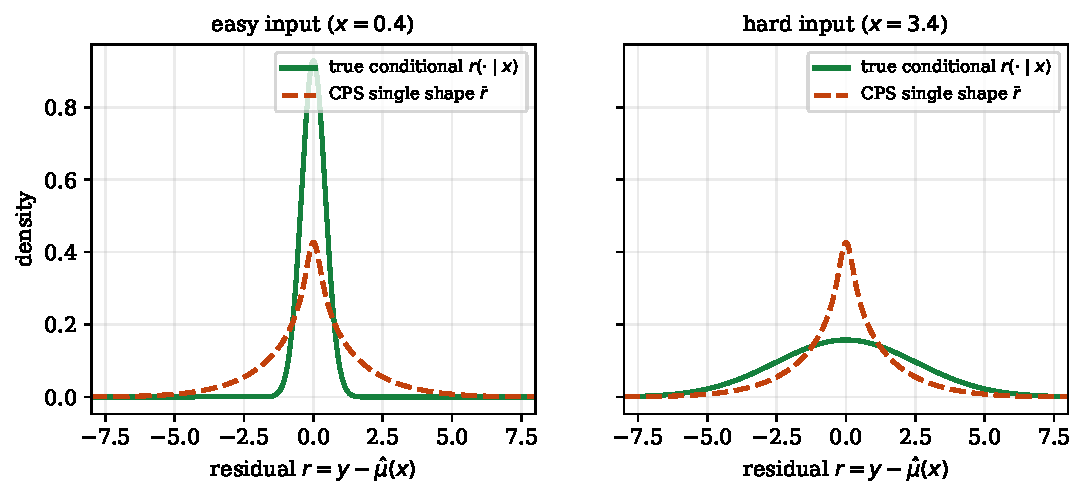
\includegraphics[width=0.92\textwidth]{figures/fig_sharpness_gap.pdf}
\caption{The residual-information gap (Propositions~\ref{prop:relevel}--\ref{prop:gap}).
A single-shape conformal predictive system uses the marginal residual law $\bar r$ for
every input; the oracle uses the true conditional $r(\cdot\given x)$, narrow for easy
inputs (left) and wide for hard ones (right). The expected log-score regret is exactly the
mutual information $I(R;X)$, which no $X$-ignoring recalibration can reduce.}
\label{fig:gap}
\end{figure}

\section{The coverage--score plane}\label{sec:plane}

The preceding results suggest a single diagnostic, provided we are careful about what is
being plotted. Define a \emph{reporting system} as a set-valued report $C_\alpha(x)$ and,
optionally, a density-valued report $f(\cdot\given x)$. Its coordinates are
\begin{equation}
  \big(\,C,\,S\,\big),\qquad
  C=\big|\,\Pr(Y\in C_\alpha(X))-(1-\alpha)\,\big|,\qquad
  S=\E[\log f(Y\given X)],
\end{equation}
the marginal-coverage error of the \emph{set} and the proper-score performance of the
\emph{density}. The decomposition of forecast quality into calibration and sharpness
\citep{gneiting2007probabilistic} is, in this plane, the statement that the two
coordinates are distinct, and our results read geometrically:
\begin{itemize}
  \item Residual split conformal is a horizontal projection. It maps a report
  $(C_\alpha^{\text{base}},f)$ to $(C_\alpha^{\text{conf}},f)$: it changes the set so that
  $C\to 0$ while leaving the density $f$ (and hence $S$) untouched
  (Proposition~\ref{prop:orth}). It moves a point left, never up.
  \item Conformal predictive systems are different: they supply their own
  density-valued report, so they do have a vertical coordinate, but that coordinate is
  governed by the single-shape restriction of Proposition~\ref{prop:gap}, capped at the
  oracle minus $I(R;X)$.
  \item Recalibration and better modeling move vertically. Fitting shape to a
  proper score raises $S$; conditioning on $x$ is the only way to raise it past the
  ceiling set by the residual-information gap \eqref{eq:gapA}.
\end{itemize}
A system reported by its coverage alone is reported by one coordinate of a
two-coordinate quality. The plane is a presentation device (adjacent to reliability
and sharpness diagrams \citep{gneiting2007probabilistic}), but the ``conformal = move
left, never up'' reading makes the category distinction hard to miss. Figure~\ref{fig:plane}
populates the plane with the time-series methods of Section~\ref{sec:exch}, using two
concrete axes: worst-window coverage (a conditional-coverage proxy) and the interval
(Winkler) score, which, like any proper score, is minimized at the oracle. The vertical axis
is therefore oriented opposite to the schematic $S$ above (down is better, not up), but the
geometry is unchanged: conformalizing moves a point horizontally, never toward a better
score.

\begin{figure}[t]
\centering

\includegraphics[width=0.78\textwidth]{figures/fig_plane.pdf}
\caption{The coverage--efficiency plane, populated by the time-series methods of
Section~\ref{sec:exch} (means over five seeds). The horizontal axis is worst rolling-window
coverage (a proxy for conditional coverage); the vertical axis is the proper interval
score. Coverage and forecast quality are distinct coordinates: the probabilistic
volatility model and the oracle dominate on score, and no method reaches per-step
conditional coverage.}
\label{fig:plane}
\end{figure}

\section{Exchangeability and the time-series case}\label{sec:exch}

Drop exchangeability and \eqref{eq:marginal} is no longer guaranteed. The literature's
repairs are ingenious, and uniform in one respect: they survive by redefining what is
guaranteed.
\begin{itemize}
  \item Weighted conformal prediction \citep{tibshirani2019conformal} restores
  marginal coverage under covariate shift when the likelihood ratio is known; with
  estimated weights coverage becomes approximate and the effective sample size drops.
  \item Adaptive Conformal Inference \citep{gibbs2021adaptive} updates the level
  online and ``puts no constraints on the data generating distribution,'' but guarantees
  a \emph{long-run time-average} miscoverage frequency,
  $\frac1T\sum_t \mathrm{err}_t\to\alpha$, not a finite-sample statement about
  $\Pr(Y\in C(X))$, and certainly not conditional coverage.
  \item EnbPI \citep{xu2021conformal} drops exchangeability for approximate
  marginal coverage under strong-mixing/stationarity surrogates; later online methods
  \citep{zaffran2022adaptive,gibbs2024conformal} retreat to regret bounds over local
  intervals. The general beyond-exchangeability analysis of \citet{barber2023conformal}
  bounds the coverage gap by a total-variation distance that is exactly what
  nonstationarity inflates.
\end{itemize}
Three distinct guarantees now travel under the word ``conformal'':
(i) \emph{split conformal under exchangeability} gives finite-sample marginal coverage;
(ii) \emph{adaptive conformal inference} gives long-run, time-average coverage control
under distribution shift; (iii) \emph{online conformal under arbitrary shifts} gives
regret-style or local-interval performance rather than the original exchangeable
guarantee. These are progressively weaker and more diffuse objects; none is the sharp
predictive distribution \emph{now}, for \emph{this} step, that a proper score grades. This
takes nothing from their utility: long-run, time-average frequency control under drift is a
genuine and hard-won engineering guarantee, often the most one can ask for without a model
of the shift. It is simply a weaker, differently posed object than conditional coverage
\emph{now}. The exchangeability required by guarantee~(i) is typically unavailable in deployed
time-series settings, though blocking or learned-transform constructions can sometimes
recover an exchangeability-like assumption.

An experiment bears this out (Figure~\ref{fig:ts}). On a
nonstationary series with known $\sigma_t$, fixed split conformal collapses far below
target once drift sets in, but the adaptive methods (ACI, conformal PID
control, and weighted/Nex\-CP) recover coverage and are competitive on the interval
(Winkler) score. They are not straw men. The finding is the one the theory predicts:
a simple probabilistic volatility model (an EWMA-variance Gaussian) matches or beats them
on the proper score \emph{and} returns a full distribution, and where the conformal methods
help they do so by adapting the interval to recently realized residuals, that
is, by local conditional modeling, with the conformal step supplying the coverage leveling
on top. Table~\ref{tab:ts} reports the main methods; full tables, including MAPIE's
EnbPI/ACI and \texttt{crepes}, are in the benchmark accompanying the paper.

\begin{figure}[t]
\centering
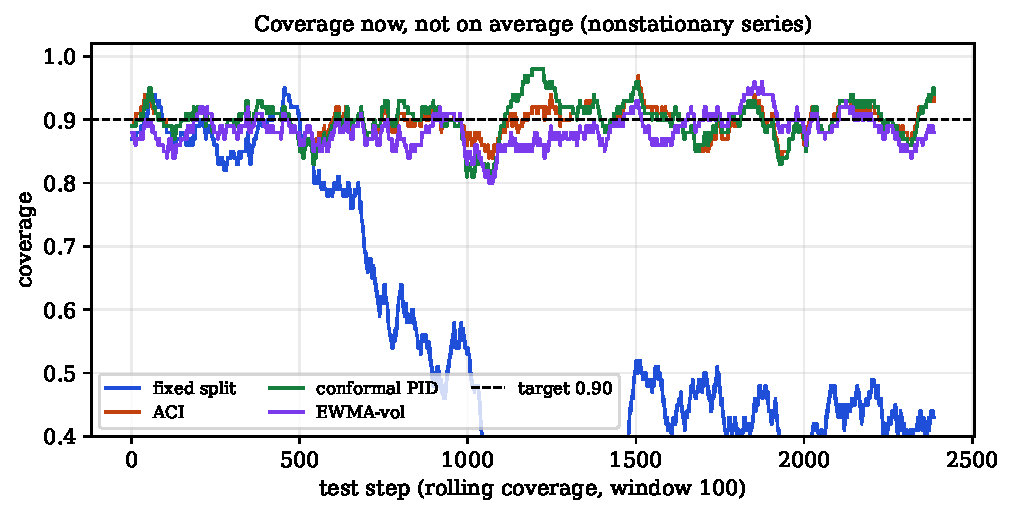
\includegraphics[width=0.82\textwidth]{figures/fig_timeseries.pdf}
\caption{Coverage now, not on average. Rolling coverage on a nonstationary series: fixed
split conformal collapses once the volatility regime arrives, while adaptive conformal
(ACI, conformal PID) and a probabilistic EWMA-volatility model track the target. Even the
recovering methods oscillate around the target rather than holding it pointwise.}
\label{fig:ts}
\end{figure}

\begin{table}[t]
\centering
\caption{Nonstationary time-series benchmark (means over five seeds; target
$1-\alpha=0.9$). Worst rolling-window coverage is a conditional-coverage proxy; the
interval (Winkler) score and CRPS are proper (lower is better); CRPS is reported only where
the method emits a density. Forecasters that model the conditional spread
(the streaming forecaster, EWMA-vol) lead on the proper score; conformalizing the best one re-levels
coverage at an essentially identical interval score ($6.58$ vs.\ $6.57$), while a naive
split-conformal wrap collapses once the regime shifts. The full table (MAPIE EnbPI/ACI,
\texttt{crepes}, GARCH, AgACI) is in the accompanying benchmark.}
\label{tab:ts}
\small
\begin{tabular}{lccccc}
\toprule
Method & Family & Marg.\ cov. & Worst-win.\ cov. & Interval score & CRPS \\
\midrule
Oracle (true $\mu,\sigma$)               & oracle & 0.900 & 0.818 & \phantom{0}5.52  & 0.76 \\
Streaming forecaster (Gaussian)          & prob.  & 0.891 & 0.700 & \phantom{0}6.57  & 0.86 \\
\quad + normalized conformal             & CP     & 0.891 & 0.694 & \phantom{0}6.58  & ---  \\
EWMA-vol Gaussian                        & prob.  & 0.886 & 0.810 & \phantom{0}6.92  & 0.92 \\
Conformal PID                            & CP     & 0.900 & 0.824 & \phantom{0}6.99  & ---  \\
ACI                                      & CP     & 0.897 & 0.830 & \phantom{0}7.00  & ---  \\
NexCP (weighted)                         & CP     & 0.884 & 0.696 & \phantom{0}7.08  & ---  \\
Streaming forecaster + split conformal   & CP     & 0.602 & 0.204 & 11.95            & ---  \\
Fixed split conformal                    & CP     & 0.562 & 0.174 & 13.82            & ---  \\
\bottomrule
\end{tabular}
\end{table}

The same holds for an off-the-shelf probabilistic forecaster. A streaming online
forecaster that emits a predictive mean and standard deviation \citep{cotton_timemachines}
has the best non-oracle interval score
($6.57$) and CRPS ($0.86$) here, because its predicted spread tracks the changing
volatility. The forecaster is deliberately simple (a fast moving average for the level
composed with a slow moving average of the
residuals for the spread), which sharpens the point: even a trivial adaptive model that
estimates conditional spread beats every conformal method here, and conformalizing it
cannot help. A normalized conformal
wrap re-levels its coverage to $1-\alpha$ at an essentially identical interval score
($6.58$ against $6.57$), and a naive split-conformal wrap on the nonstationary series
collapses (to $60\%$ coverage, score $11.9$). The conformal step re-levels. It does not
add sharpness, which is the experience the introduction describes.

\section{When coverage \emph{is} the objective}\label{sec:steel}

The argument is skeptical, not dismissive, and it comes with a precise converse. The
litmus is one question:
\begin{quote}
\emph{Is your loss a function of \emph{whether} the truth lands in a region, or of
\emph{where} it lands?}
\end{quote}
If the former, coverage is the native object and conformal prediction is sound and often
ideal:
\begin{itemize}
  \item Selective prediction and risk control. ``Return a small set guaranteed
  to contain the label $95\%$ of the time; a human checks it.'' The deliverable is a set;
  risk-controlling prediction sets and conformal risk control formalize this
  \citep{angelopoulos2021uncertainty, bates2021distribution, angelopoulos2024conformalrisk}.
  \item Retrieval and shortlisting, where the product is a candidate set and
  coverage is recall.
  \item Anomaly and novelty detection via conformal $p$-values, conformal
  prediction's most natural home, because here it is not a forecaster but a
  distribution-free hypothesis test and coverage is Type-I error control
  \citep{vovk2005algorithmic}.
  \item Compliance and long-run frequency control, where a certificate of the
  form ``contained $95\%$ of the time on average'' \emph{is} the product, and the
  distribution-free, finite-sample nature of \eqref{eq:marginal} is exactly the value
  added.
\end{itemize}
Two caveats temper even these. If you trust a calibrated posterior you can form a
sharper set yourself (the smallest region of mass $\ge 1-\alpha$) and recover the
expectations a bare set discards; conformal's marginal value is then purely the
distribution-free guarantee, useful when you distrust the density and exchangeability
holds. And even when coverage is the goal you usually want it conditionally, which
returns us to the impossibility of Section~\ref{sec:marginal}.

\section{Scope, and the constructive escapes}\label{sec:scope}

Our strong claims target the object that is actually over-sold: \emph{post-hoc, marginal,
split conformal prediction with a residual score}. A large and active literature builds
conformal methods that do more; the conditional constructions below (CQR, Mondrian / binned
CPS) are by now standard practice, not niche alternatives, and we do not question their
effectiveness. How they relate still matters, because in every case they confirm the paper's
mechanism rather than contradict it: they buy sharpness or conditional coverage by
\emph{conditioning on $X$ or optimizing a proper objective}, which is exactly what
Proposition~\ref{prop:gap} says is required --- that is, by modeling, rather than by anything
the conformal step itself supplies.

\paragraph{Conformal predictive systems that condition on $X$.}
Mondrian / binned conformal predictive systems \citep{bostrom2021mondrian} fit a separate
residual law per region, and \citet{toccaceli2026crps} chooses the bins by minimizing a
leave-one-out CRPS. These produce sharp, shape-adaptive predictive
distributions, and they do so by leaving the single-shape class of
Proposition~\ref{prop:relevel} (a per-bin shape is $X$-dependent) and, in the CRPS case,
by making the partition criterion a proper score. This is the most pointed case for the
defence, and the concession is real: when the reference class is itself selected by
a proper scoring rule, the conformal \emph{construction} is performing conditional density
estimation. The category distinction does not vanish; it relocates to ``which component
estimates the distribution,'' and the answer is the conditional partition, not the
coverage certificate: the value is in the estimation, as throughout. Conformalized
quantile regression \citep{romano2019conformalized} is the same story with a quantile
model in place of the bins.

\paragraph{End-to-end conformal training.}
The orthogonality of Proposition~\ref{prop:orth} is a statement about \emph{post-hoc}
conformalization of a fixed predictor. Conformal training
\citep{stutz2022learning,correia2024information} deliberately differentiates through the
conformalizer to minimize expected set size subject to coverage, which couples the
coverage and efficiency axes by construction. This does not contradict the proposition; it
illustrates its corollary: to obtain sharpness you must optimize for it, rather than
read it off the coverage certificate.

\paragraph{The information in set size.}
\citet{correia2024information} connect conformal set size to information-theoretic
uncertainty, with bounds relating expected prediction-set size to the conditional entropy
$H(Y\mid X)$. This is complementary to our
Proposition~\ref{prop:gap}: both say conformal \emph{geometry} carries information. It also
sharpens the two-coordinate plane of Section~\ref{sec:plane}: the \emph{efficiency}
(set-size / sharpness) coordinate is the information-bearing one, while the marginal
\emph{coverage} coordinate, by Proposition~\ref{prop:orth}, is not. Reporting only the
latter discards exactly the coordinate that encodes aleatoric uncertainty.

\paragraph{Approaching conditional coverage.}
The no-go result of Section~\ref{sec:marginal} concerns \emph{exact, distribution-free,
finite-length} conditional coverage. It is not the end of the subject. Diagnostics such as
the excess-risk-of-target-coverage family \citep{braun2025conditional} quantify and
decompose the conditional gap; methods that target conditional or subgroup-wise validity
directly interpolate between marginal and conditional coverage \citep{gibbs2025conditional};
and post-processing via pivotal scores and optimal transport
\citep{laplante2026pivotal} attains \emph{approximate} conditional coverage by estimating
the conditional law of the score, again conditioning on $X$, and explicitly under the
structural assumptions the impossibility theorem rules out for the exact, assumption-free
case. These approach the goalpost; they do not move the one the no-go result defends.

\paragraph{Modern time-series conformal.}
Beyond the adaptive methods benchmarked in Section~\ref{sec:exch}, methods such as HopCPT
\citep{auer2023hopcpt} exploit temporal structure to tighten intervals and improve
empirical adaptivity. Their guarantees remain of the approximate / long-run kind catalogued
there; the improvement, again, comes from modeling the conditional error law.

\paragraph{Beyond the log-score.}
We used the log-score for the clean information-theoretic identities. The two-coordinate
distinction (coverage versus score) carries over to any strictly proper score, but the exact
mutual-information identity is special to the log-score; for CRPS or the interval score the
analogous gap is the regret of the best $X$-blind residual law under that score. The
accompanying benchmark in fact ranks methods by the interval (Winkler) score and CRPS
\citep{gneiting2007strictly}, on which the same orderings hold.

\section{Prediction versus verification}\label{sec:verification}
Conformal prediction \emph{verifies} a coverage property. It does not \emph{model}, and a
fixed rule cannot substitute for modeling. Conformalization is best viewed as a terminal
certification operator: it repairs the marginal coverage coordinate of a set-valued report,
but any improvement in a proper score must come from upstream modeling of the conditional
location, scale, quantiles, or residual shape. It moves only the coverage coordinate; the
residual-information gap is reduced only by conditioning on $X$ (the conditional-shape models
of Section~\ref{sec:scope}), never by the conformal step.

\paragraph{Practical remarks.} (i) Conformalize \emph{last}: model first, then add the
certificate, since the conformal step cannot improve any proper score (estimate first, certify
second). (ii) Use a proper score (log-likelihood, CRPS) as the sharpness diagnostic; because
conformalization leaves it unchanged, a score that does not move after conformalizing confirms
that any gain came from modeling. (iii) To close $I(R;X)$, add conditioning to the model
(heteroscedastic spread, quantile or residual-shape estimation), not tightness to the
conformal step.

\paragraph{Limitations.} The exact result is deliberately narrow, and we state where it
stops. (i) \emph{Scope.} The strong claims concern post-hoc, marginal, split conformal with
a residual score and the single-shape residual class; the conditional constructions of
Section~\ref{sec:scope} (CQR, Mondrian/binned CPS, conformal training) leave that class by
design and are out of scope as targets of the critique. (ii) \emph{Fixed location.} The gap
$I(R;X)$ is defined for a fixed $\hat\mu$ and measures conditional residual shape, not the
quality of the point forecast (Remark~\ref{rem:mudep}). (iii) \emph{Score-specific
identity.} The exact mutual-information form is special to the log-score; for CRPS or the
interval score the analogous gap is the regret of the best $X$-blind residual law under that
score, not an information quantity. (iv) \emph{Asymptotic density statement.} The
density/log-score equalities of Propositions~\ref{prop:relevel}--\ref{prop:gap} are a
large-calibration (or smoothed-density) statement; the object conformal delivers
finite-sample is coverage, not a density. (v) \emph{Synthetic illustrations.} The figures
and benchmark use synthetic generators with known ground truth, which is what makes the
oracle and $I(R;X)$ computable; the identity itself is verified numerically by
\texttt{check\_gap.py}.

\section{Conclusion}

Conformal prediction certifies the coverage of a set, finite-sample and
distribution-free, under exchangeability. That guarantee is genuine and, for the right
objective, exact. The error is reading it as distributional forecast quality. For a fixed
location predictor, the guarantee you can have (marginal) is rarely the one you want
(conditional), and the conditional one is not available distribution-free without more
structure. The output is a set, not a measure. Read as a single-shape distribution, its
log-score loss against the oracle is exactly the residual-information term
$I(R;X)$ of \eqref{eq:gapA}. And the exchangeability even the basic guarantee needs is
usually missing in deployed time-series. Within the single-shape residual class it is
optimal, and where a guarantee is the product it is the right tool. But coverage answers a question,
\emph{is the truth in this region?}, that, in forecasting, is often not the one you
were asking. Conformal prediction is not weak uncertainty quantification. It is exact
uncertainty quantification for a set --- a coverage guarantee, no more and no less. The
category error is reading that certificate as a verdict on the forecast underneath it.

\paragraph{Reproducibility.} Every figure is generated by the accompanying script
\texttt{figures.py} (Figures~\ref{fig:nogo}--\ref{fig:ts}), and the time-series experiment
by the benchmark scripts, all from the synthetic generators described in the text. The
identities of Proposition~\ref{prop:gap} are confirmed numerically by \texttt{check\_gap.py},
which computes both sides independently (by grid integration) and matches them to machine
precision on a heteroscedastic Gaussian and a skewed residual law. Code, figures, and an
interactive companion are provided as supplementary material; public URLs are omitted for
double-blind review.

\subsubsection*{Broader Impact Statement}
This is a theoretical clarification of what a conformal-prediction coverage guarantee does
and does not entail. It introduces no new models, data, or deployment, and we foresee no
direct ethical risks; if anything, being precise about the limits of a widely used
uncertainty tool reduces the risk of its being over-trusted.

\bibliographystyle{tmlr}
\bibliography{references}

\end{document}
